\documentclass{bmstu}
\usepackage[]{svg}
\usepackage[]{pdfpages}
\usepackage{multirow}
\usepackage{amsmath}
\usepackage{graphicx}
\usepackage{appendix}

\newcounter{myfigure}
\pretocmd{\figure}{\stepcounter{myfigure}}{}{}
\renewcommand{\thefigure}{\arabic{myfigure}}
\newcounter{mytable}
\pretocmd{\table}{\stepcounter{mytable}}{}{}
\renewcommand{\thetable}{\arabic{mytable}}

\renewcommand{\theequation}{\arabic{equation}}

\setenumerate[1]{label={ \arabic*)}}
\NewBibliographyString{accessmode}
\DeclareFieldFormat{url}{\bibstring{accessmode}\addcolon\space\url{#1}}
\DeclareFieldFormat{title}{#1}
\DefineBibliographyStrings{russian}{
accessmode={Режим доступа:},
urlseen={дата обращения:}
}
\captionsetup[table]{justification=raggedright,singlelinecheck=off}
\renewcommand\labelitemi{---}

\bibliography{biblio}

\begin{document}
% \renewcommand{\thelstlisting}{\arabic{lstlisting}}

% \makecourseworktitle
%     {Информатика и системы управления}
%     {Программное обеспечение ЭВМ и информационные технологии}
%     {Разработка базы данных электронной образовательной платформы}
%     {~П.~А. Шпаковский/ИУ7-63Б}
%     {~Т.~А. Никульшина}
%     {}

\setcounter{page}{3}
\maketableofcontents

\chapter*{Введение}
\addcontentsline{toc}{chapter}{ВВЕДЕНИЕ}

В современном мире электронные образовательные платформы становятся все более популярными и широко используются для обучения и самосовершенствования. Автоматизация анализа информации об обучающихся, курсах, материалах и результатов обучения на таких платформах играет ключевую роль в обеспечении эффективного функционирования системы. В связи с увеличением количества создаваемых обучающих материалов, актуальной задачей становится разработка системы управления образовательной деятельностью, а также обеспечение безопасности и целостности данных.

Цель данной работы -- разработка базы данных электронной образовательной платформы.

Чтобы достичь поставленной цели, требуется решить следующие задачи: 
\begin{itemize}
    \item проанализировать существующие решения;
    \item спроектировать базу данных;
    \item спроектировать приложение доступа к базе данных;
    \item реализовать приложение доступа к базе данных;
    \item исследовать зависимость времени проверки целостности данных на уровне приложения и базы данных от количества записей в таблице.
\end{itemize}

\chapter{Аналитическая часть}

В данной части проводится анализ существующих решений, формализация данных, ролей и задачи, анализ баз данных.

\section{Анализ существующих решений}
На рынке онлайн образования представлено множество платформ, предоставляющих образовательные материалы разной тематики и формы. Ключевым критерием, по которому были отобраны существующие решения, является наличие на платформе как теории, так и практики. При анализе отобранных решений были выделены следующие критерии:
\begin{itemize}
    \item наличие подробного отчета о пройденном обучении;
    \item возможность создать и опубликовать на платформе собственный курс;
    \item понятный и простой пользовательский интерфейс;
    \item возможность основать собственную школу.
\end{itemize}

\begin{table}[H]
    \caption{\label{tbl:alternatives}Сравнение существующих решений}
	\resizebox{\textwidth}{!}{
	\def\arraystretch{1}
    \begin{tabular}{|c|c|c|c|c|}
    \hline
    Решение          & Подробный отчет & Создание курса & Собственная школа & Простой польз. интерфейс \\ \hline
    Stepik           & +               & +              & -                 & +                        \\ \hline
    Coursera         & -               & -              & -                 & -                        \\ \hline
    Яндекс Практикум & +               & -              & -                 & +                        \\ \hline
    \end{tabular}%
    }
\end{table}

Из таблицы \ref{tbl:alternatives} видно, что существующие решения не удовлетворяют описанным требованиям в полной мере.

\section{Формализация данных}
В предметной области онлайн образования ключевыми сущностями являются школа и курс. Школа в данной работе включает в себя множество преподавателей, студентов и курсов, которые могут быть реализованы
преподавателями данной школы. Также школа содержит дополнительную информацию о создателе, платежные данные
для оплаты того или иного курса и прочую дополнительную информацию.

Каждый курс разбит на уроки, которые могут быть нескольких типов: текстовые, видео-уроки и практические.
Текстовые и видео уроки предоставляют теоретические знания, в то время как практические задания
реализуются в виде тестов с множественным выбором.

База данных должна хранить информацию о следующих сущностях:
\begin{itemize}
    \item пользователи;
    \item школы;
    \item курсы;
    \item уроки, принадлежащие некоторому курсу;
    \item практические тесты;
    \item отзывы;
    \item сертификаты.
\end{itemize}

На рисунке \ref{img:er} приведена ER-диаграмма сущностей в нотации Чена.

\begin{figure}[H]
	\centering
	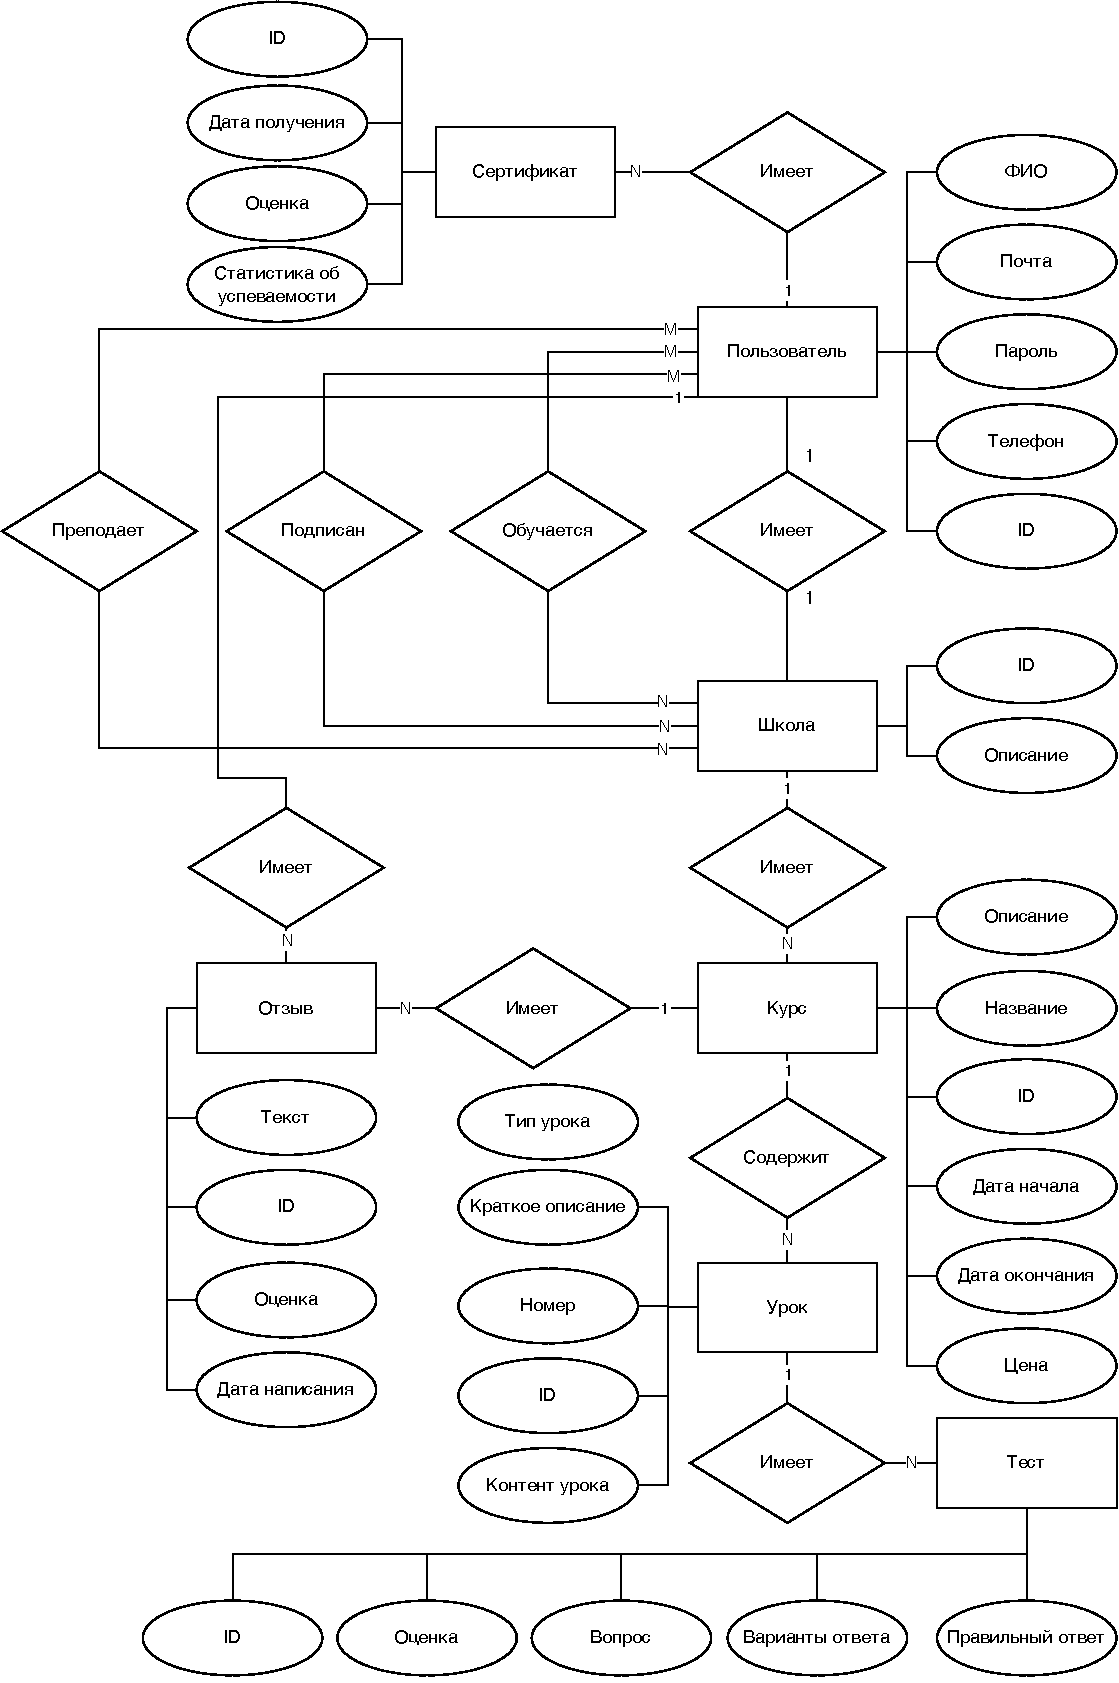
\includegraphics[height=0.9\textheight]{inc/img/er.pdf}
	\caption{ER-диаграмма сущностей в нотации Чена}
	\label{img:er}
\end{figure}

\section{Формализация ролей}
В данной работе выделяются следующие роли пользователей:
\begin{itemize}
    \item гость -- неавторизованный пользователь, который может посматривать информацию о курсе,
    авторизоваться, зарегистрироваться;
    \item пользователь -- авторизованный пользователь, может просматривать курсы, проходить, оплачивать их,
    по завершении курса получать сертификат и отчет об успеваемости и оставлять отзывы,
    стать преподавателем, создать собственную школу и курсы в ней,
    а также присоединиться к существующей школе в качестве преподавателя;
    \item администратор -- авторизованный пользователь, может создавать, изменять и удалять пользователей, курсы, школы, уроки, отзывы.
\end{itemize}

\section{Формализация задачи}
Необходимо спроектировать базу данных для хранения информации о студентах и преподавателях, школах, курсах и уроках, входящих в состав курса, а также об отзывах пользователей.
Разработанное приложение для доступа к базе данных должно предоставлять каждому пользователю возможность покупать и проходить курсы различной тематики. Также у каждого пользователя должна быть возможность создать собственную школу и образовательную программу
или присоединиться к уже существующей школе в качестве преподавателя или составителя курса.

По прохождении курса пользователь должен иметь возможность получить сертификат о завершении обучения,
включающий подробное описание его успеваемости и итоговую оценку. Диаграмма вариантов использования приведена на рисунке \ref{img:usecase}.

\begin{figure}[H]
	\centering
	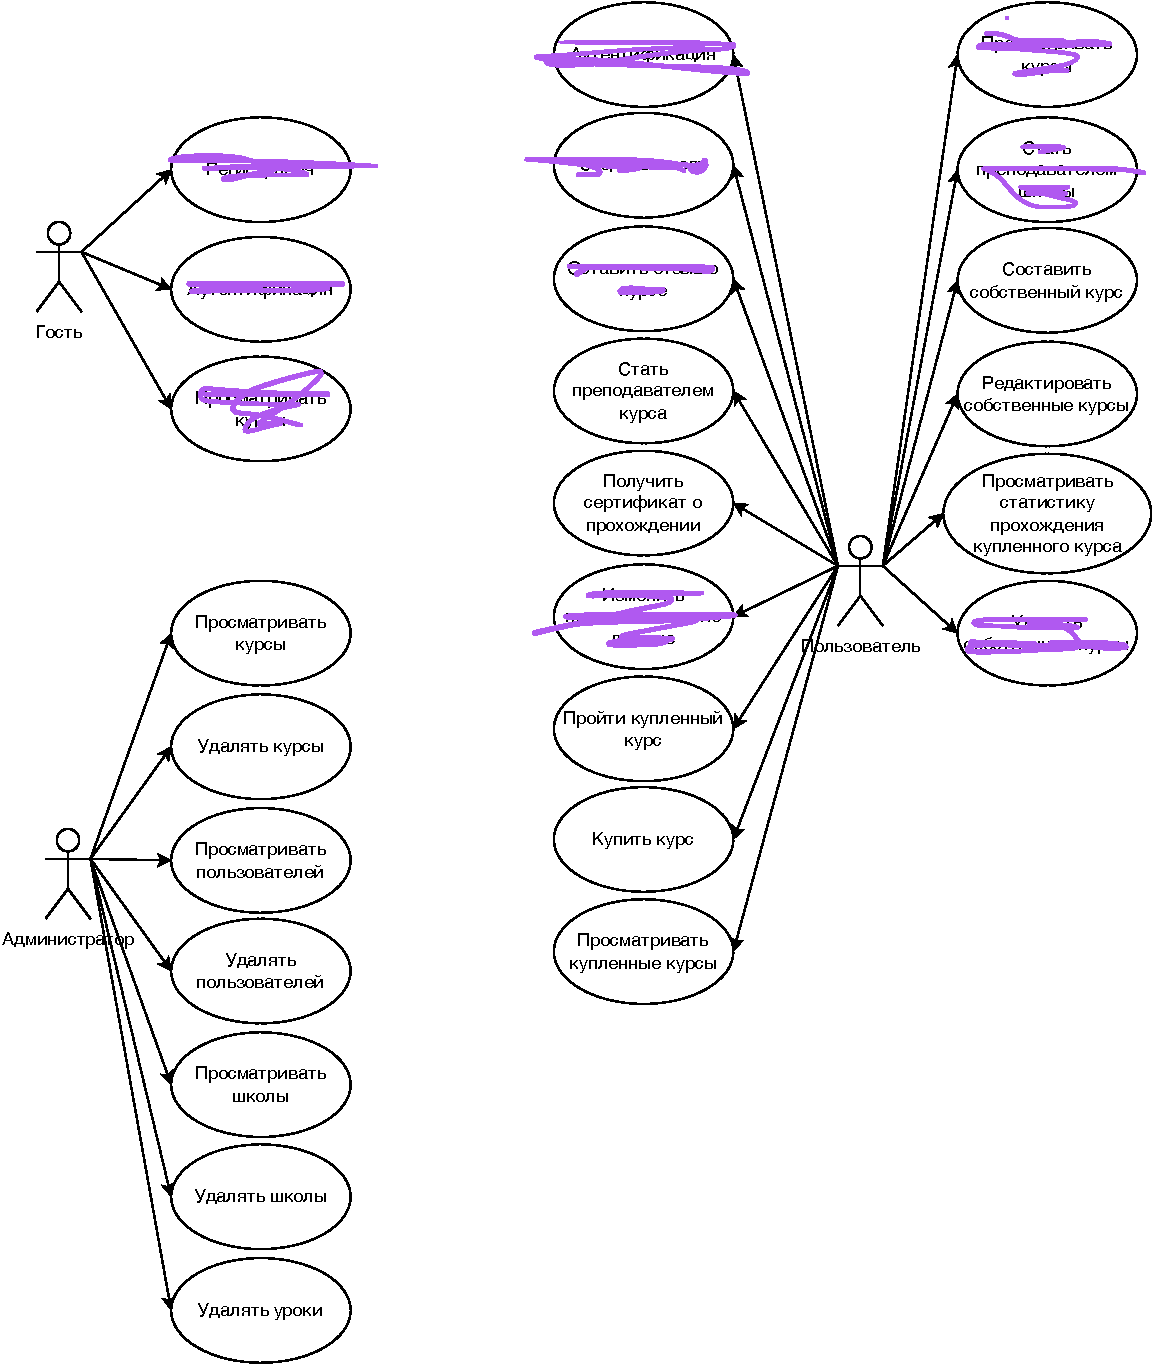
\includegraphics[height=0.7\textheight]{inc/img/usecase.pdf}
	\caption{Диаграмма вариантов использования}
	\label{img:usecase}
\end{figure}

\section{Анализ баз данных}
База данных -- совокупность данных, хранимых в соответствии со схемой данных, манипулирование которыми выполняют в соответствии с правилами средств моделирования данных.

СУБД -- совокупность языковых и программных средств общего или специального назначения, обеспечивающих управление созданием и использованием баз данных~\cite{williams}.

Модель данных представляет собой абстрактное, логическое описание элементов, таких как объекты и операции, которые в совокупности образуют виртуальную систему управления данными, с которой взаимодействует пользователь. Объекты модели описывают структуру данных, в то время как операции отражают их поведение.

Базы данных можно классифицировать по модели хранения на несколько типов:
\begin{itemize}
    \item дореляционные модели данных --- включают иерархические, сетевые модели и системы, использующие инвертированные списки.
    \item реляционные модели данных --- основываются на таблицах, что делает их более гибкими и простыми в использовании.
    \item нереляционные модели данных --- ориентированы на расширенные возможности работы с данными, выходящие за рамки реляционной парадигмы.
\end{itemize}

\subsection*{Дореляционные модели}
Дореляционные базы данных представляют собой тип баз данных, который не использует табличную модель данных. Вместо этого, они хранят данные в структурах, таких как деревья, графы или объекты. 

\subsection*{Реляционная модель данных}
Реляционные базы данных основаны на реляционной модели данных, где данные организованы в виде таблиц, которые имеют связи между собой. Каждая таблица представляет отдельную сущность, а связи между таблицами устанавливаются с помощью ключевых полей. Важным свойством реляционных баз данных является их способность удовлетворять требованиям ACID~\cite{acid}: атомарность, согласованность, изоляция, устойчивость. Примерами реляционных баз данных являются MySQL~\cite{mysql}, PostgreSQL~\cite{postgres}, Oracle~\cite{oracle} и SQL Server~\cite{sql-server}.

\subsection*{Нереляционная модель данных}
Постреляционные базы данных -- это базы данных, которые разработаны для обработки и анализа больших объемов данных. В отличие от реляционных баз данных, основанных на таблицах, нереляционные базы данных предлагают более гибкие способы хранения данных, что делает их подходящими для определенных типов задач, таких как обработка больших объемов данных, работа с распределенными системами и требование высокой производительности. Примерами постреляционных баз данных являются Apache Hadoop~\cite{hadoop}, Apache Cassandra~\cite{cassandra} и Apache Spark~\cite{spark}.

\section{Вывод из аналитической части}
С учетом задачи была выбрана реляционная модель хранения данных, так как предметная область может быть представлена в виде таблиц и должна удовлетворять требованиям ACID.

\chapter{Конструкторская часть}

В данной части будет представлена схема проектируемой базы данных, будут описаны сущности базы данных, ограничения целостности, ролевая модель и используемые функции и триггеры.

\section{Диаграмма проектируемой базы данных}

На рисунке \ref{img:scheme} представлена диаграмма проектируемой базы данных.

\begin{figure}[H]
	\centering
	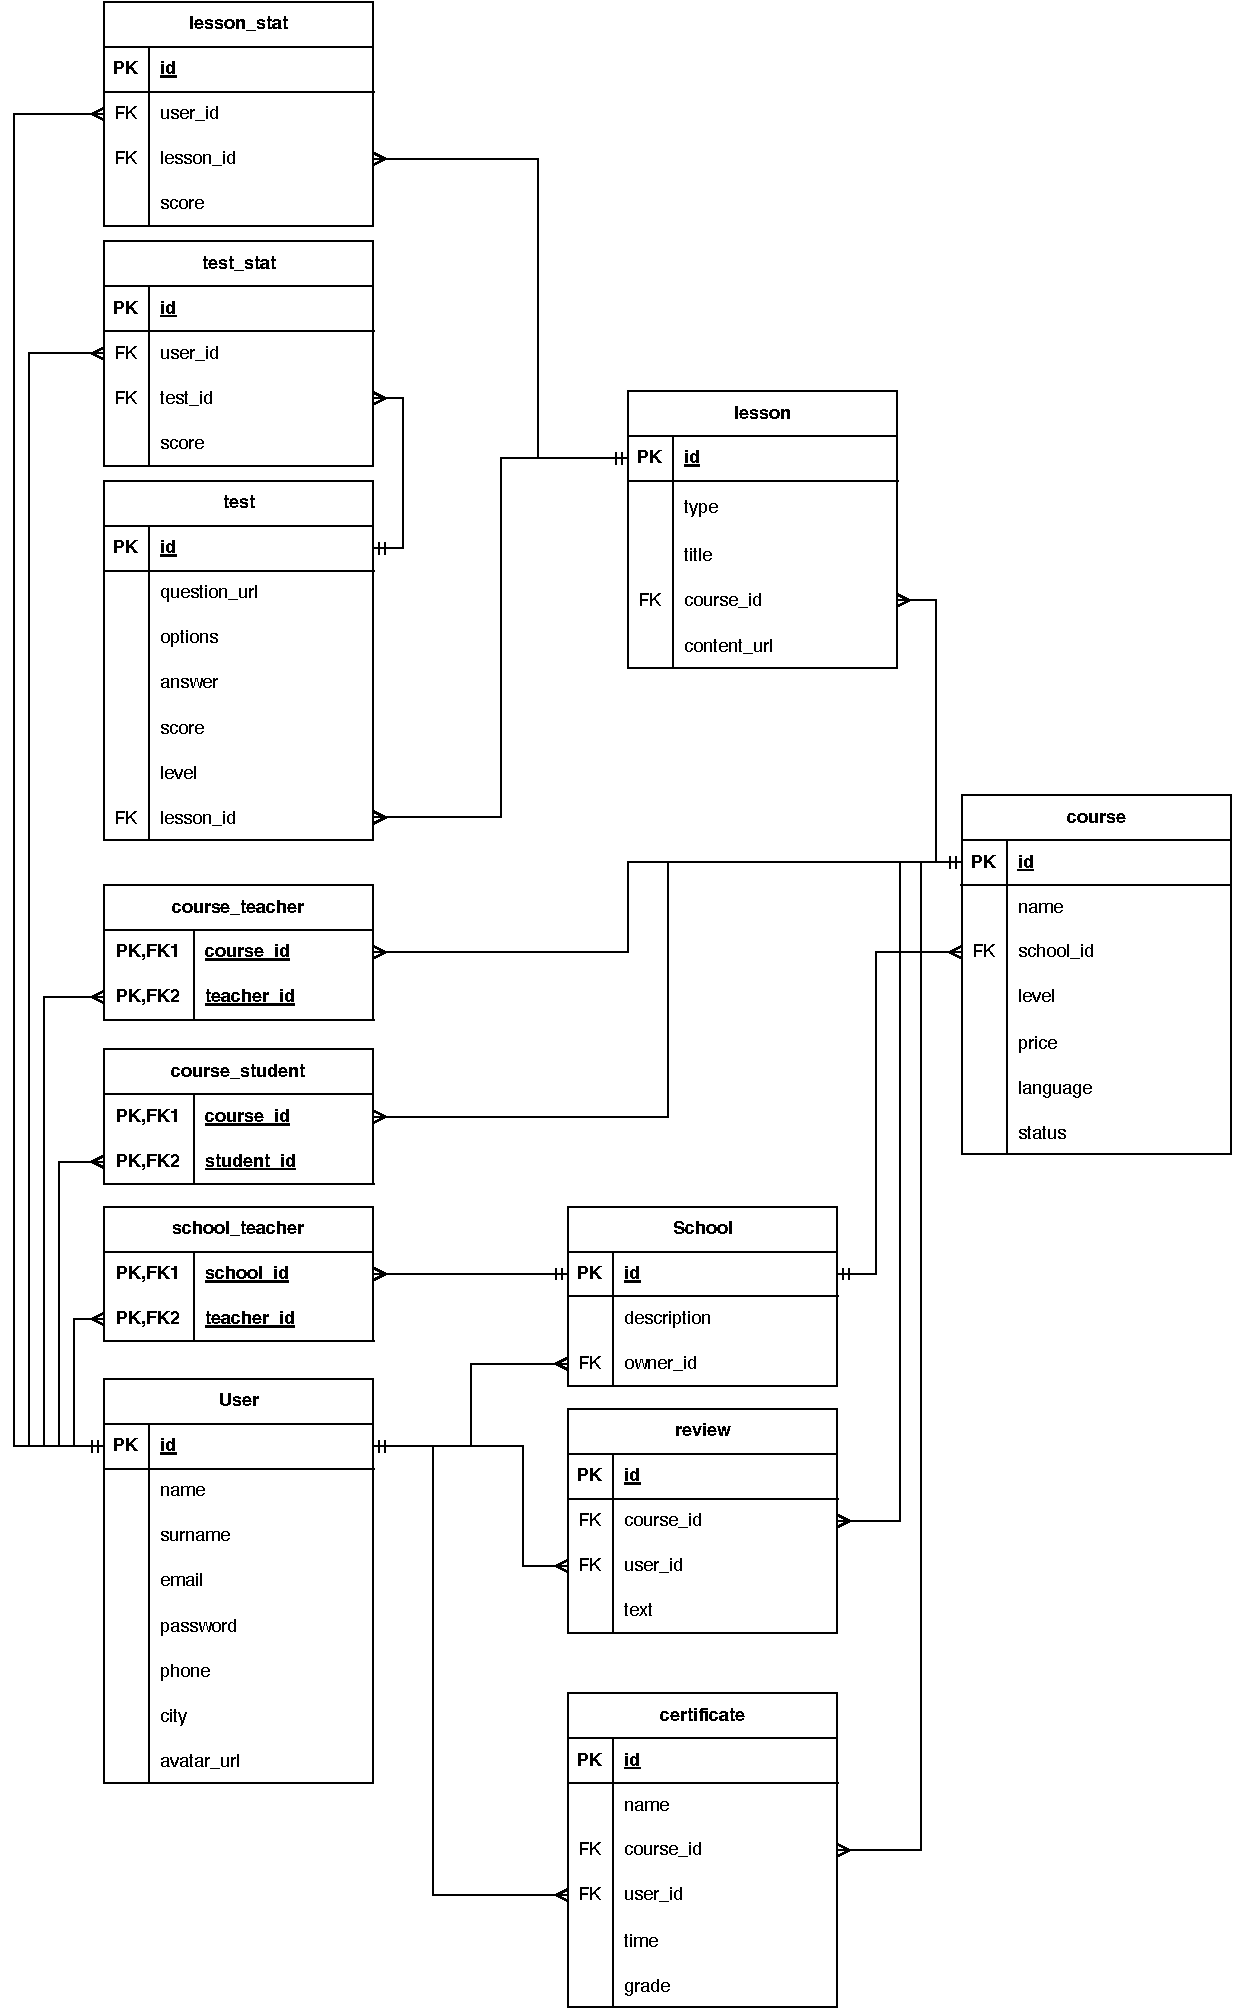
\includegraphics[height=0.9\textheight]{inc/img/scheme.pdf}
	\caption{Диаграмма проектируемой базы данных}
	\label{img:scheme}
\end{figure}

\section{Описание сущностей базы данных}


\begin{table}[H]
	\caption{\label{tbl:user}Поля таблицы user}
	\resizebox{\textwidth}{!}{
	\def\arraystretch{1}
	\begin{tabular}{|l|l|l|l|}
	\hline
	Поле        & Тип данных   & Ограничения целостности & Описание                      \\ \hline
	id          & uuid         & primary key             & Идентификатор пользователя    \\ \hline
	email       & varchar(255) & unique not null         & Почта пользователя            \\ \hline
	password    & varchar(255) & not null                & Пароль пользователя           \\ \hline
	name        & varchar(255) & not null                & Имя пользователя              \\ \hline
	surname     & varchar(255) & not null                & Фамилия пользователя          \\ \hline
	phone       & varchar(255) & нет                     & Номер телефона пользователя   \\ \hline
	city        & varchar(255) & нет                     & Город пользователя            \\ \hline
	avatar\_url & text         & нет                     & Ссылка на аватар пользователя \\ \hline
	\end{tabular}
	}
\end{table}

\begin{table}[H]
	\caption{\label{tbl:school}Поля таблицы school}
	\resizebox{\textwidth}{!}{
	\def\arraystretch{1}
	\begin{tabular}{|l|l|l|l|}
	\hline
	Поле        & Тип данных   & Ограничения целостности & Описание                      \\ \hline
	id          & uuid         & primary key             & Идентификатор школы    \\ \hline
	name        & varchar(255) & not null                & Название школы                \\ \hline
	description & text         & not null                & Описание школы                \\ \hline
	owner\_id   & uuid         & not null                & Идентификатор владельца школы \\ \hline
	\end{tabular}
	}
\end{table}

\begin{table}[H]
	\caption{\label{tbl:course}Поля таблицы course}
	\resizebox{\textwidth}{!}{
	\def\arraystretch{1}
	\begin{tabular}{|l|l|l|l|}
	\hline
	Поле       & Тип данных     & Ограничения целостности & Описание                                                                        \\ \hline
	id         & uuid           & primary key             & Идентификатор курса                                                             \\ \hline
	name       & varchar(255)   & not null                & Название курса                                                                  \\ \hline
	school\_id & uuid           & not null                & \begin{tabular}[c]{@{}l@{}}Идентификатор школы,\\ владеющей курсом\end{tabular} \\ \hline
	level      & int            & not null                & Уровень сложности курса                                                         \\ \hline
	price      & bigint         & not null                & Цена курса                                                                      \\ \hline
	language   & varchar(255)   & not null                & Язык материала курса                                                            \\ \hline
	status     & course\_status & not null                & Текущий статус курса                                                            \\ \hline
	rating     & float          & not null                & Пользовательская средняя оценка курса                                                   \\ \hline
	\end{tabular}
	}
\end{table}

Поле status таблицы school имеет перечисляемый тип данных и может принимать три варианта: <<draft>>, <<ready>>, <<published>>. Статус курса -- текущее состояние готовности и наполнения материалом курса. Черновик курса может редактироваться автором, после чего может быть переведен в состояние готовности к публикации. После успешной публикации курса, состояние меняется на <<опубликован>>.

\begin{table}[H]
	\caption{\label{tbl:lesson}Поля таблицы lesson}
	\resizebox{\textwidth}{!}{
	\def\arraystretch{1}
	\begin{tabular}{|l|l|l|l|}
	\hline
	Поле        & Тип данных   & Ограничения целостности & Описание                                                                             \\ \hline
	id          & uuid         & primary key             & Идентификатор урока                                                                  \\ \hline
	title       & varchar(255) & not null                & Название урока                                                                       \\ \hline
	type        & lesson\_type & not null                & Тип урока                                                                            \\ \hline
	score       & int          & not null                & Максимальная оценка за урок                                                          \\ \hline
	theory\_url & text         & нет                     & \begin{tabular}[c]{@{}l@{}}Ссылка на теоретический \\ материал урока\end{tabular}    \\ \hline
	video\_url  & text         & нет                     & Ссылка на видео материал урока                                                       \\ \hline
	course\_id  & uuid         & not null                & \begin{tabular}[c]{@{}l@{}}Идентификатор курса,\\ который содержит урок\end{tabular} \\ \hline
	\end{tabular}
	}
\end{table}

Урок может быть трех видов: теоретический, видео-урок и практический урок. Тип урока описывается полем type таблицы lesson и может принимать значения: <<theory>>, <<video>>, <<practice>>.

\begin{table}[H]
	\caption{\label{tbl:test}Поля таблицы test}
	\resizebox{\textwidth}{!}{
	\def\arraystretch{1}
	\begin{tabular}{|l|l|l|l|}
	\hline
	Поле       & Тип данных & Ограничения целостности & Описание                                                                            \\ \hline
	id         & uuid       & primary key             & Идентификатор теста                                                                 \\ \hline
	task\_url  & text       & not null                & \begin{tabular}[c]{@{}l@{}}Ссылка на описание \\ задачи теста\end{tabular}          \\ \hline
	options    & text       & not null                & Возможные варианты ответа                                                           \\ \hline
	answer     & text       & not null                & Ответ на задание                                                                    \\ \hline
	score      & int        & not null                & \begin{tabular}[c]{@{}l@{}}Максимальная оценка за \\ прохождение теста\end{tabular} \\ \hline
	level      & int        & not null                & Уровень сложности теста                                                             \\ \hline
	lesson\_id & uuid       & not null                & \begin{tabular}[c]{@{}l@{}}Идентификатор урока, \\ содержащего тест\end{tabular}    \\ \hline
	\end{tabular}
	}
\end{table}

\begin{table}[H]
	\caption{\label{tbl:review}Поля таблицы review}
	\resizebox{\textwidth}{!}{
	\def\arraystretch{1}
	\begin{tabular}{|l|l|l|l|}
	\hline
	Поле       & Тип данных & Ограничения целостности & Описание                      \\ \hline
	id         & uuid       & primary key             & Идентификатор отзыва об уроке \\ \hline
	text       & text       & not null                & Текст отзыва об уроке         \\ \hline
	course\_id & uuid       & not null                & Идентификатор курса           \\ \hline
	user\_id   & uuid       & нет                     & Идентификатор пользователя    \\ \hline
	rating     & int        & нет                     & Оценка курса                  \\ \hline
	\end{tabular}
	}
\end{table}

\begin{table}[H]
	\caption{\label{tbl:certificate}Поля таблицы certificate}
	\resizebox{\textwidth}{!}{
	\def\arraystretch{1}
	\begin{tabular}{|l|l|l|l|}
	\hline
	Поле        & Тип данных         & Ограничения целостности & Описание                          \\ \hline
	id          & uuid               & primary key             & Идентификатор отзыва об уроке     \\ \hline
	name        & varchar(1024)      & not null                & Название сертификата              \\ \hline
	score       & int                & not null                & Итоговая оценка прохождения курса \\ \hline
	grade       & certificate\_grade & not null                & Степень сертификата               \\ \hline
	created\_at & timestamp          & not null                & Дата выдачи сертификата           \\ \hline
	user\_id    & uuid               & not null                & Идентификатор пользователя        \\ \hline
	course\_id  & uuid               & нет                     & Идентификатор курса               \\ \hline
	\end{tabular}
	}
\end{table}

Сертификаты могут быть трех видов: бронзовый, серебряный и золотой. Тип сертификата описывается полем grade таблицы certificate и может принимать значения: <<bronze>>, <<silver>>, <<gold>>.

\begin{table}[H]
	\caption{\label{tbl:lesson_stat}Поля таблицы lesson\_stat}
	\resizebox{\textwidth}{!}{
	\def\arraystretch{1}
	\begin{tabular}{|l|l|l|l|}
	\hline
	Поле       & Тип данных & Ограничения целостности & Описание                                                                                       \\ \hline
	id         & uuid       & primary key             & \begin{tabular}[c]{@{}l@{}}Идентификатор записи о \\ результате прохождения урока\end{tabular} \\ \hline
	score      & int        & not null                & Оценка прохождения урока                                                                       \\ \hline
	user\_id   & uuid       & not null                & Идентификатор пользователя                                                                     \\ \hline
	lesson\_id & uuid       & not null                & Идентификатор урока                                                                            \\ \hline
	\end{tabular}
	}
\end{table}

\begin{table}[H]
	\caption{\label{tbl:test_stat}Поля таблицы test\_stat}
	\resizebox{\textwidth}{!}{
	\def\arraystretch{1}
	\begin{tabular}{|l|l|l|l|}
	\hline
	Поле     & Тип данных & Ограничения целостности & Описание                                                                                       \\ \hline
	id       & uuid       & primary key             & \begin{tabular}[c]{@{}l@{}}Идентификатор записи о \\ результате прохождения урока\end{tabular} \\ \hline
	score    & int        & not null                & Оценка прохождения урока                                                                       \\ \hline
	user\_id & uuid       & not null                & Идентификатор пользователя                                                                     \\ \hline
	test\_id & uuid       & not null                & Идентификатор тест                                                                             \\ \hline
	\end{tabular}
	}
\end{table}

Таблицы lesson\_stat и test\_stat хранят данные о прохождении пользователем уроков и тестов соответственно. Сертификат о прохождении курса формируется на основании информации из этих таблиц. 

\begin{table}[H]
	\caption{\label{tbl:course_student}Поля таблицы course\_student}
	\resizebox{\textwidth}{!}{
	\def\arraystretch{1}
	\begin{tabular}{|l|l|l|l|}
	\hline
	Поле        & Тип данных & Ограничения целостности & Описание                   \\ \hline
	student\_id & uuid       & not null                & Идентификатор пользователя \\ \hline
	course\_id  & uuid       & not null                & Идентификатор курса        \\ \hline
	\end{tabular}
	}
\end{table}

\begin{table}[H]
	\caption{\label{tbl:course_teacher}Поля таблицы course\_teacher}
	\resizebox{\textwidth}{!}{
	\def\arraystretch{1}
	\begin{tabular}{|l|l|l|l|}
	\hline
	Поле        & Тип данных & Ограничения целостности & Описание                   \\ \hline
	teacher\_id & uuid       & not null                & Идентификатор пользователя \\ \hline
	course\_id  & uuid       & not null                & Идентификатор курса        \\ \hline
	\end{tabular}
	}
\end{table}

\begin{table}[H]
	\caption{\label{tbl:school_teacher}Поля таблицы school\_teacher}
	\resizebox{\textwidth}{!}{
	\def\arraystretch{1}
	\begin{tabular}{|l|l|l|l|}
	\hline
	Поле        & Тип данных & Ограничения целостности & Описание                   \\ \hline
	teacher\_id & uuid       & not null                & Идентификатор пользователя \\ \hline
	school\_id  & uuid       & not null                & Идентификатор школы        \\ \hline
	\end{tabular}
	}
\end{table}

Таблица course\_student является развязочной для курсов и обучающихся на них студентах. Развязочная таблица course\_teacher связывает курсы и их преподавателей, а таблица school\_teacher является развязочной для школ и их преподавателей.

\section{Ролевая модель}

В данной работе выделяются следующие роли:
\begin{itemize}
	\item гость -- имеет возможность просматривать курсы, школы и их преподавателей, отзывы о курсах;
	\item пользователь -- имеет права на просмотр, редактирование и удаление собственных курсов, школ, уроков, тестов, а также может проходить приобретенные курсы;
	\item администратор -- имеет все права для действий со всеми таблицами.
\end{itemize}

\section{Триггер базы данных}

К каждому курсу пользователи, прошедшие данный курс, могут оставить отзыв и выставить оценку качества. При этом средняя оценка курса должна меняться при операциях над таблицей отзывов. Для этого используется триггер базы данных, который сработает при добавлении, удалении или обновлении отзыва пользователя. Таким образов, средняя оценка пересчитывается и при получении информации о курсе исчезает необходимость пересчитывать ее каждый раз.

На рисунке \ref{img:trigger} представлена схема алгоритма триггера для пересчета средней оценки курса.

\begin{figure}[H]
	\centering
	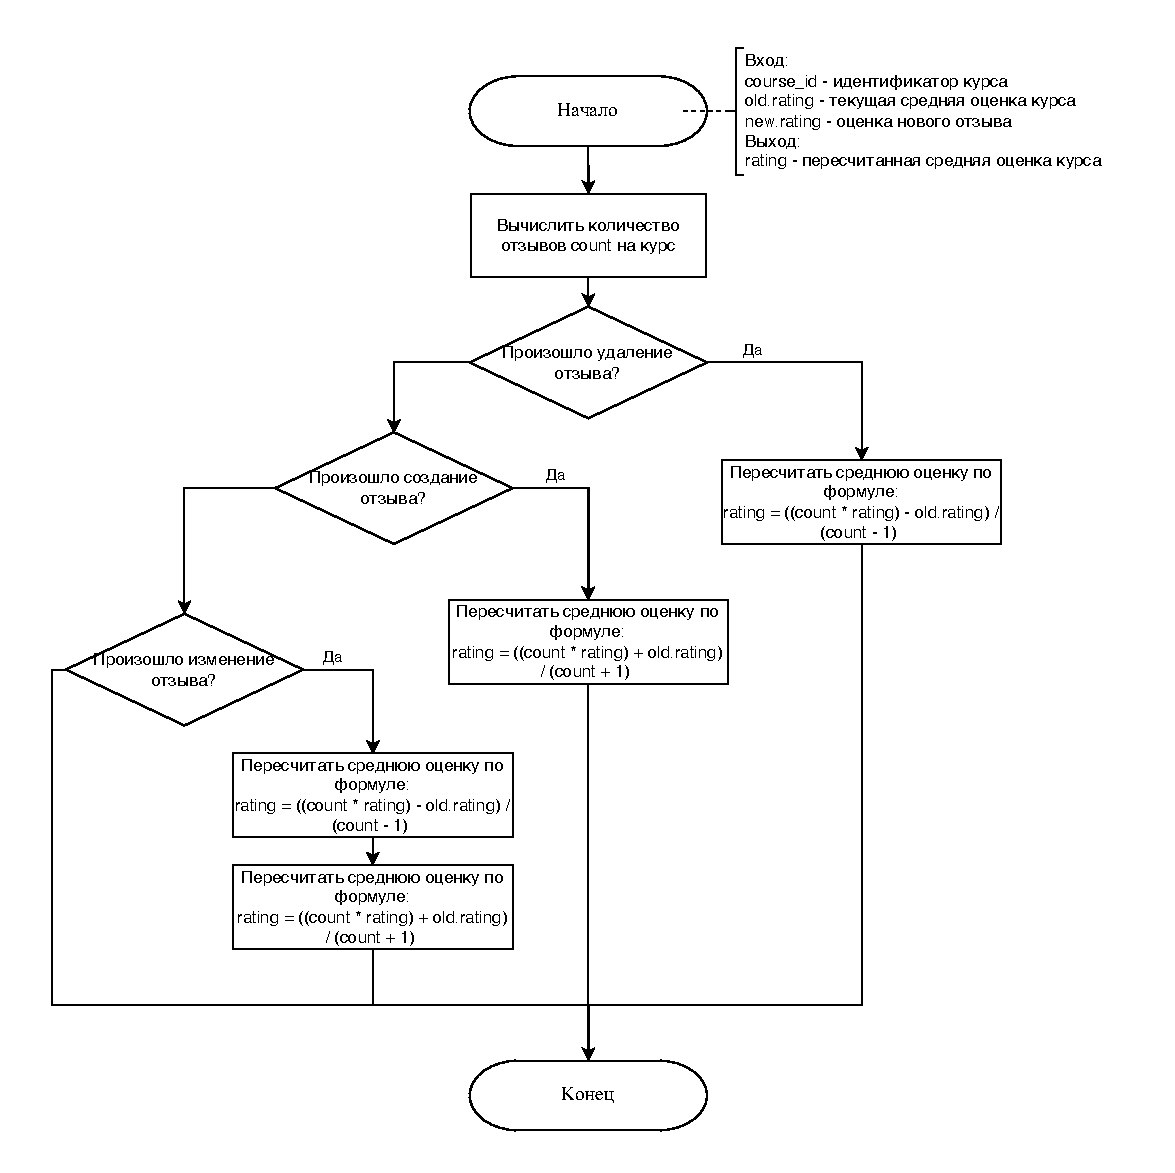
\includegraphics[height=0.7\textheight]{inc/img/trigger.pdf}
	\caption{Схема алгоритма триггера}
	\label{img:trigger}
\end{figure}

\section{Вывод из конструкторской части}

В данной части были спроектирована схема базы данных, описаны сущности базы данных, ограничения целостности, ролевая модель и используемые функции и триггеры.

\chapter{Технологическая часть}

В данной части приводится обоснование выбора СУБД и средств реализации приложения для взаимодействия с базой данных. Также приводится реализация создания таблиц базы данных, реализация ролевой модели на уровне базы данных и реализация триггера. Кроме того описаны методы тестирования разработанного функционала и приведена реализация интерфейса доступа к базе данных.

\section{Выбор системы управления базами данных}

Чтобы выбрать СУБД необходимо рассмотреть следующие критерии:
\begin{itemize}
    \item бесплатное и открытое программное обеспечение;
    \item поддержка процедурных расширений языка SQL;
    \item наличие личного опыта работы.
\end{itemize}

\begin{table}[H]
    \caption{\label{tbl:dbms}}
	\resizebox{\textwidth}{!}{
	\def\arraystretch{1}
    \begin{tabular}{|l|c|c|c|}
    \hline
    \begin{tabular}[c]{@{}l@{}}Система управления \\ базами данных\end{tabular} &
      \multicolumn{1}{l|}{\begin{tabular}[c]{@{}l@{}}Бесплатное и открытое \\ программное обеспечение\end{tabular}} &
      \multicolumn{1}{l|}{\begin{tabular}[c]{@{}l@{}}Поддержка процедурных \\ расширений языка SQL\end{tabular}} &
      \multicolumn{1}{l|}{\begin{tabular}[c]{@{}l@{}}Наличие личного \\ опыта работы\end{tabular}} \\ \hline
    PostgreSQL~\cite{postgres} & + & + & + \\ \hline
    Oracle~\cite{oracle}     & - & + & - \\ \hline
    SQLite~\cite{sqlite}     & + & + & - \\ \hline
    \end{tabular}
    }
\end{table}

По таблице \ref{tbl:dbms} можно сделать вывод, что наиболее подходящей СУБД для данной работы является PostgreSQL.

\section{Выбор объектного хранилища}

Объектное хранилище --- это тип системы хранения данных, предназначенный для управления большими объемами неструктурированной информации, такой как мультимедийные файлы, бэкапы, лог-файлы, документы и другие типы данных. Вместо традиционной файловой системы или реляционной базы данных, объектное хранилище организует данные в виде <<объектов>>.

Для хранения файлов с материалами создаваемых преподавателями курсов необходимо использовать объектное хранилище. При этом в базе данных должны храниться ссылки на получение данных файлов пользователем курса. 

Amazon S3~\cite{s3} --- одно из самых популярных облачных хранилищ с поддержкой API, множеством классов хранения и глобальной инфраструктурой для высокой доступности. Данное хранилище не доступно на территории РФ, поэтому использование его в данной работе невозможно. 

Google Cloud Storage~\cite{google-cloud} --- это облачная служба хранения данных от Google, предназначенная для хранения и управления большими объёмами неструктурированных данных. Это объектное хранилище, которое позволяет загружать, сохранять и извлекать данные любого типа, например, мультимедийные файлы, резервные копии, журналы, архивы, документы и многое другое. Данное хранилище доступно в РФ, однако услуги, предоставляемые компанией платные.

MinIO~\cite{minio} --- это программное обеспечение с открытым исходным кодом, которое позволяет создавать объектные хранилища, совместимые с API Amazon S3. MinIO часто используется для развертывания облачных хранилищ на локальных серверах, в частных или гибридных облаках. 

Учитывая доступность объектных хранилищ на территории РФ, их стоимость и наличие личного опыта работы, было выбрано хранилище MinIO для взаимодействия с файлами материалов курсов преподавателей. 

\section{Средства реализации}

В данной работе использованы следующие средства реализации:
\begin{itemize}
    \item язык программирования Golang~\cite{go};
    \item СУБД PostgreSQL~\cite{postgres};
    \item расширение языка SQL PL/pgSQL~\cite{pgsql};
    \item автоматизация развертывания реализована с помощью Docker~\cite{docker}.
\end{itemize}

Доступ к базе данных реализован в виде консольного интерфейса. Тестирование функционала проводилось с помощью встроенной программы go test~\cite{go-test}.

\section{Создание таблиц базы данных}

В листинге \ref{lst:scheme.sql} приведена реализация создания таблиц для сущностей предметной области.

\section{Создание ролей базы данных}

В листинге \ref{lst:roles.sql} приведена реализация создания ролей базы данных.

\pagebreak
\section{Реализация триггера}

В листинге \ref{lst:trigger.sql} приведена реализация триггера для пересчета средней оценки курса.

\includelisting
    {trigger.sql}
    {Реализация триггера}

\pagebreak
\section{Интерфейс доступа к базе данных}

В листинге \ref{lst:interface.txt} приведен пример пользовательского интерфейса.

\includelisting
    {interface.txt}
    {Консольный интерфейс приложения}

\section{Тестирование разработанного функционала}

В процессе тестирования были использованы два подхода: модульное тестирование и интеграционное. Модульное тестирование проводилось с помощью стандартного пакета testing~\cite{go-test} языка golang. Для изоляции сервисного слоя приложения использовался подход mock тестирования~\cite{mock-testing} и библиотека Mockery~\cite{mockery}.

Интеграционное тестирование уровня доступа к базе данных проводилось с использованием библиотеки Testcontainers~\cite{testcontainers}. 

На рисунке \ref{img:tests} изображены результаты пройденных тестов и их количество.

\begin{figure}[H]
	\centering
	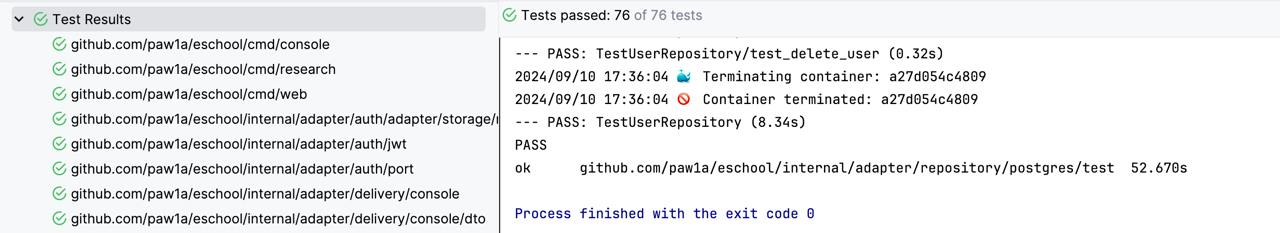
\includegraphics[height=0.12\textheight]{inc/img/tests.jpeg}
	\caption{Результаты пройденных тестов разработанного функционала}
	\label{img:tests}
\end{figure}

\section{Вывод из технолгической части}

В данной части была выбрана используемая СУБД и средства реализации приложения для взаимодействия с базой данных, приведена реализация создания таблиц базы данных, реализация ролевой модели на уровне базы данных и триггера. Были представлены методы тестирования разработанного функционала и пример реализации интерфейса доступа к базе данных.

\chapter{Исследовательская часть}

В данной части будет проводено исследование разработанных алгоритмов компьютерной графики для использования их с применением аппаратных возможностей микроконтроллера. 

Целью исследования является определение зависимости времени выполнения классического и модифицированного алгоритмов Варнока от количества визуализируемых полигонов на сцене, а также сравнение данных алгоритмов. Замеры времени проводятся для количества полигонов, изменяющегося от 50 до 500 с шагом измерения в 50 полигонов. 

\section{Средства реализации}
При проведении исследования используется микроконтроллер RP2040~\cite{rp2040} в плате Raspberry Pi Pico. Для отображения итогового изображения используются два экрана с разрешением 240x240 пикселов, подключенные по одной шине SPI. 

Характеристики микроконтроллера RP2040:
\begin{itemize}
    \item 32-битный процессор ARM Cortex-M0+~\cite{cortex-m0};
    \item тактовая частота процессора -- 133 МГц;
    \item объем оперативной памяти -- 264 Кб;
    \item объем постоянной памяти -- 2 Мб;
    \item частота шины SPI -- 40 МГц;
    \item наличие встроенного контроллера DMA~\cite{dma}. 
\end{itemize}

Для замера времени работы реализованных алгоритмов используется системый системный таймер SysTick~\cite{systick}, который является частью процессоров семейства Cortex-M. 

\section{Результаты исследования}
В таблице \ref{tbl:time} приведены результаты замеров времени для двух реализаций алгоритма Варнока удаление невидимых граней.

\begin{table}[H]
    \caption{\label{tbl:time}Замеры времени сравнения алгоритмов Варнока}
	\resizebox{\textwidth}{!}{
	\def\arraystretch{1}
    \begin{tabular}{|c|c|c|}
    \hline
    Кол-во полигонов, шт &
      \begin{tabular}[c]{@{}c@{}}Модифицированный \\ алгоритм Варнока, мс\end{tabular} &
      \begin{tabular}[c]{@{}c@{}}Классический \\ алгоритм Варнока, мс\end{tabular} \\ \hline
    50  & 1452  & 2032  \\ \hline
    100 & 3132  & 4698  \\ \hline
    150 & 5076  & 7360  \\ \hline
    200 & 6349  & 8903  \\ \hline
    250 & 9071  & 12699 \\ \hline
    300 & 10865 & 14124 \\ \hline
    350 & 12168 & 18435 \\ \hline
    400 & 15323 & 22984 \\ \hline
    450 & 17342 & 23744 \\ \hline
    500 & 19891 & 29836 \\ \hline
    \end{tabular}
    }
\end{table}

На рисунке \ref{img:plot} представлен график зависимости времени работы двух алгоритмов Варнока в зависимости от заданного количества полигонов.

\begin{figure}[H]
	\centering
	\includegraphics[height=0.35\textheight]{inc/img/plot.pdf}
	\caption{Сравнение классического и модифицированного алгоритмов Варнока}
	\label{img:plot}
\end{figure}

\section{Вывод из исследовательской части}
В результате исследования можно заметить, что модифицированный алгоритм Варнока превосходит классическую реализацию алгоритма по эффективности. Таким образом, за счет использования аппаратных особенностей микроконтроллера удалось достичь меньшего времени визуализации сцены. Прямой доступ к памяти обеспечивает более эффективный доступ к периферии, при этом нагрузка на процессор не увеличивается.

\chapter*{Заключение}
\addcontentsline{toc}{chapter}{ЗАКЛЮЧЕНИЕ}

В ходе выполнения данной курсовой работы были выполнены следующие задачи:
\begin{itemize}
    \item проанализированы существующие решения;
    \item спроектирована база данных;
    \item спроектировано приложение доступа к базе данных;
    \item реализовано приложение доступа к базе данных;
    \item исследована зависимость времени проверки целостности данных на уровне приложения и базы данных от количества записей в таблице.
\end{itemize}


\makebibliography

\chapter*{Приложение А}
\addcontentsline{toc}{chapter}{ПРИЛОЖЕНИЕ А}
\section*{Презентация к курсовой работе}


\end{document}
